\chapter{Context \& Requirements\label{cha:chapter4}}
The goal of this Master Thesis is to complete the implementation of the Zk-Rollup project, test it under different conditions, evaluate its performances and finally show a proof of concept of the system applied to a real world application. This will bring a good understanding of the rollup system and show how it can be used and applied to other minor blockchain without many adaptations. This differs to other scaling solutions, like the ones described in \cite{yang_review_2020}, because they are developed closely to the blockchain they are applied to, limiting the future possibility to extend that solution.

\section{ADSP Project: Scaling Tezos Blockchain with Zk-Rollups \label{sec:2_adspProject}}

In the Winter Semester 2022/2023 at the University of Berlin, I collaborated with the ADSP (Advanced Distributed Systems Prototype) group on a project. The project's objective was to scale the Tezos blockchain using Zk-Rollups through the ZoKrates toolbox.

The group partially achieved the project's objectives, creating a proof of concept. The system architecture features Layer 1 and Layer 2 components: Layer 1 includes two smart contracts for state management and proof verification; Layer 2 encompasses a node executing transactions within the ZoKrates program, generating proofs for the smart contract. Figure \ref{fig:3_general_rollup_architecture} offers an overview of the entire system.

\begin{figure}[ht]
  \centering
  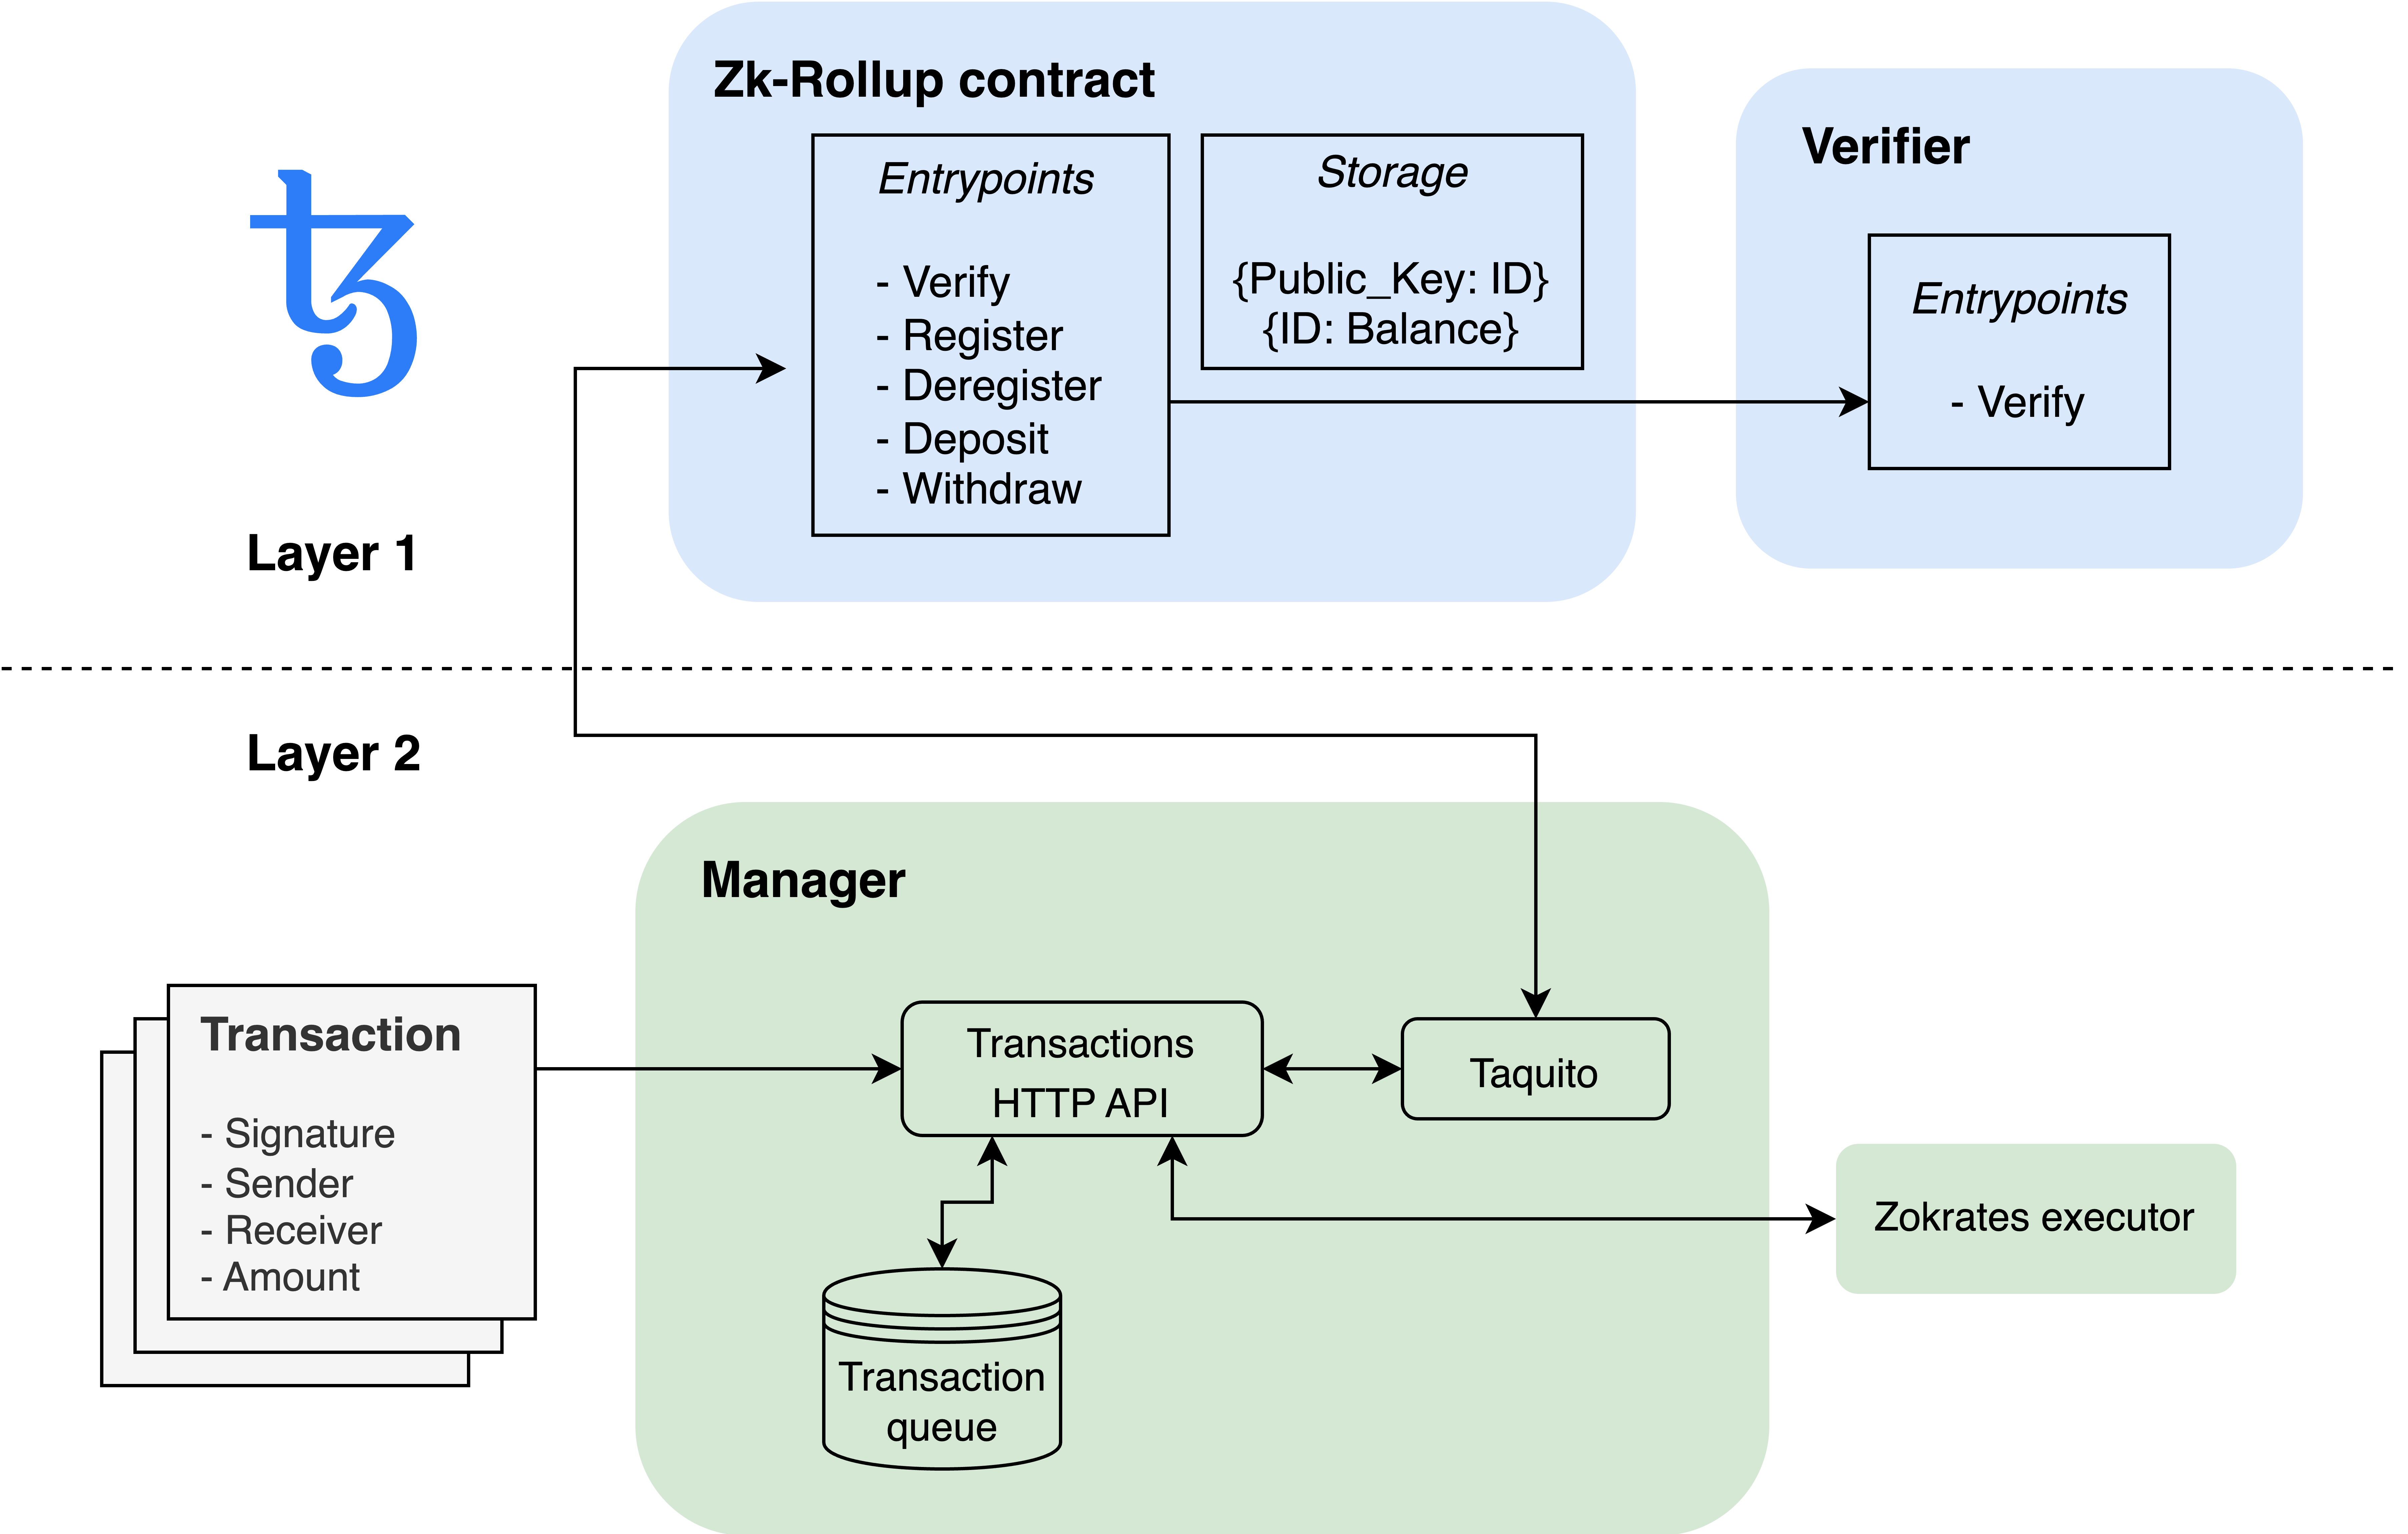
\includegraphics[width=0.95\columnwidth]{2_drawings-adsp_rollup_architecture.png}
  \caption[Project Architecture]{Project architecture}  
  \label{fig:3_general_rollup_architecture}
\end{figure}

The Zk-Rollup execution process occurs as follows:
\begin{enumerate}
    \item A user dispatches a transaction to the off-chain node, managed by a NodeJS server (the Web-Manager);
    \item The Web-Manager logs the transaction in a transaction queue;
    \item Once three transactions accumulate, the Web-Manager fetches the current state from the Tezos Zk-Rollup smart contract;
    \item The L2 node processes the transaction batch, executing the ZoKrates program using the transaction batch and the current state as input;
    \item The ZoKrates program generates a proof and new balance list;
    \item The node converts ZoKrates outputs into a Tezos-compatible format;
    \item Converted outputs are dispatched to the Tezos Rollup smart contract using Taquito, an external Typescript library;
    \item The smart contract forwards the proof to the verifier smart contract;
    \item The verifier smart contract verifies the proof, communicating the result to the Rollup-Manager contract;
    \item If the proof is verified, the new balance list is stored in the Manager contract's blockchain storage.
\end{enumerate}

Figure \ref{fig:3_drawings-adsp_sequence_general.png} illustrates the sequence of events in the Zk-Rollup execution process.

\begin{figure}[ht]
  \centering
  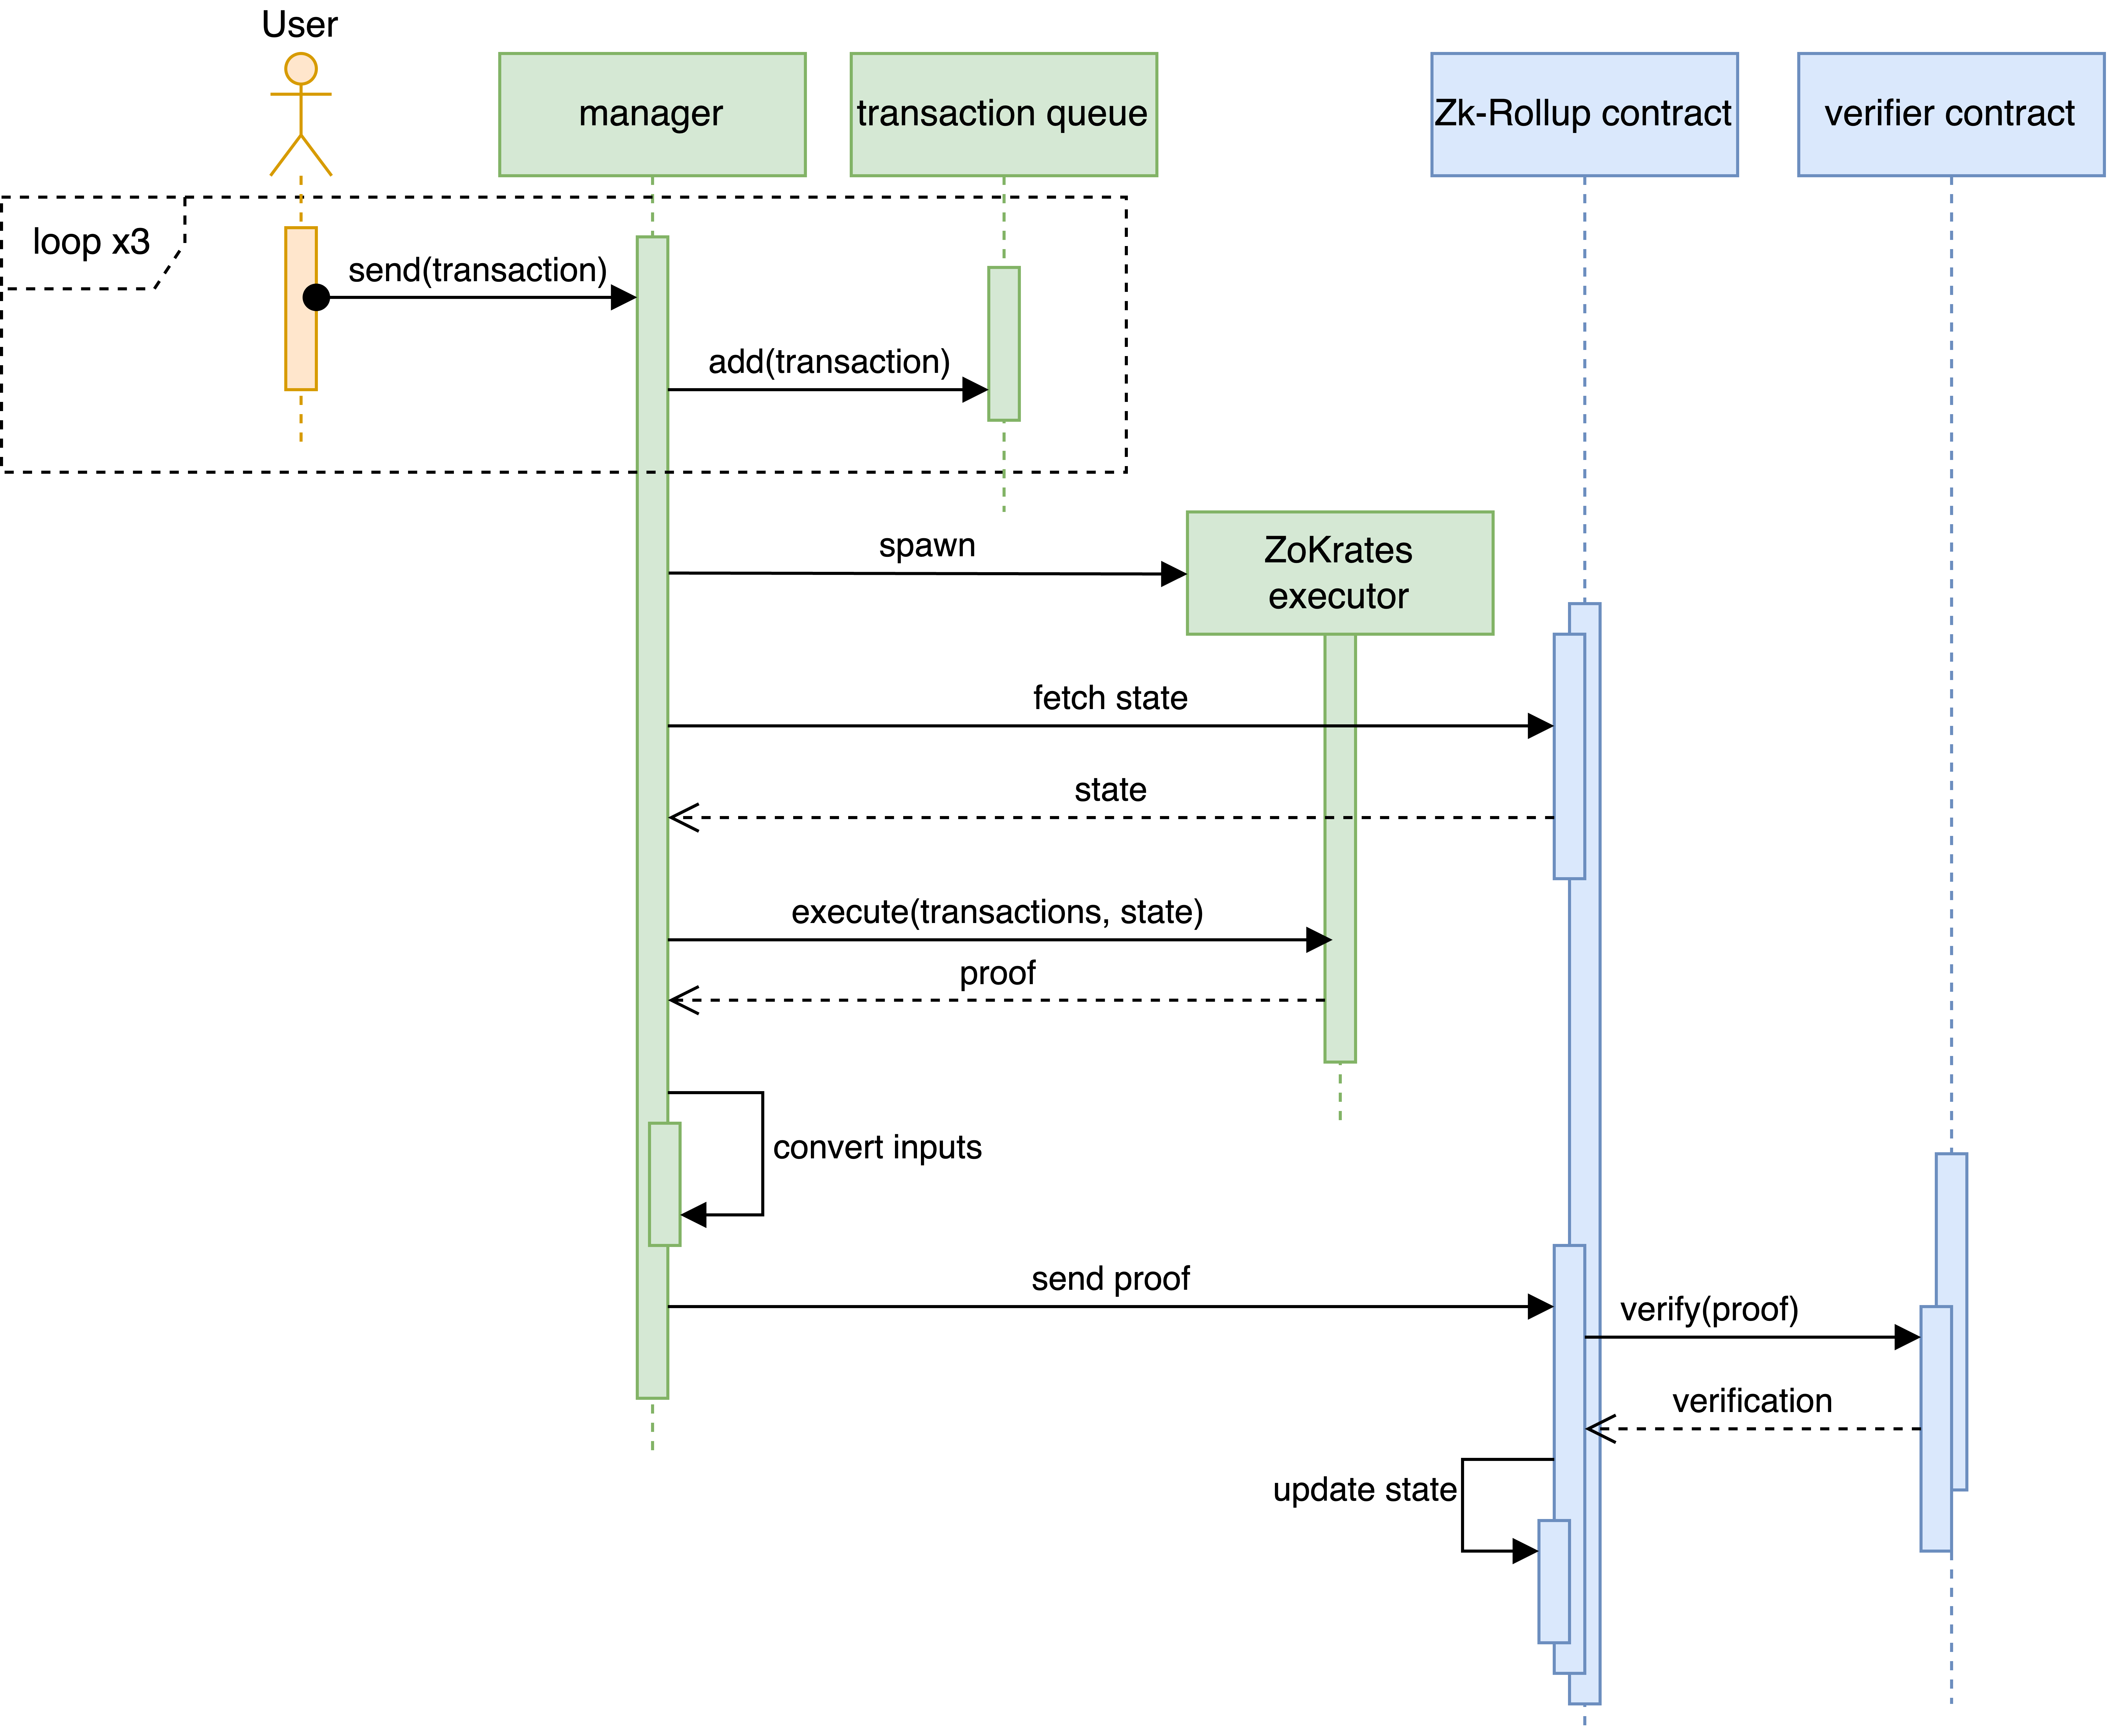
\includegraphics[width=1\columnwidth]{2_drawings-adsp_sequence_general.png}
  \caption[Sequence Zk-Rollup]{Sequence diagram of the Zk-Rollup execution process.}  
  \label{fig:3_drawings-adsp_sequence_general.png}
\end{figure} 

\subsection{Developed Components}
The team successfully implemented the Rollup-Manager \textit{Verify} entrypoint within the \textit{Rollup contract}, along with the \textit{NodeJS Manager}. Additionally, the storage mechanism was correctly executed.

The ZoKrates program was partially developed, including:
\begin{itemize}
    \item Verification of account inclusion in the rollup system;
    \item Verification of sufficient balance in sender account;
    \item Transaction execution;
    \item Generation of new balance merkle tree root, balance list, and proof.
\end{itemize}

The generation of the Merkle tree root is accomplished through the algorithm described below. This process utilizes the SHA2-256 hash function with automatic zero-padding. The algorithm incorporates pre-calculated values for the Merkle tree depth and the number of leaf nodes.

\noindent\textbf{Algorithm 1: Merkle Tree Root Generation}
\begin{lstlisting}[language=Python]
for i in 0...TREE_DEPTH {
  step_size = 2 ** (i + 1)
  step_number = LEAFS_NUM / step_size
  for j in 0...step_number {
    leftIndex = j * step_size
    rightIndex = leftIndex + step_size / 2
    leafs[leftIndex] = hash(
        leafs[leftIndex],
        leafs[rightIndex]
    )
  }
}
return leafs[0]
\end{lstlisting}

\subsection{Pending Components\label{subsec:pendingcomponents}}
Numerous aspects of the project remain unfinished, including:
\begin{itemize}
  \item Registration entrypoint;
  \item Deregistration entrypoint;
  \item Deposit entrypoint;
  \item Withdrawal entrypoint;
  \item Integration of signature checks within the ZoKrates program;
  \item Addressing the double spending issue;
  \item System optimization.
\end{itemize}
Furthermore, the project lacks a benchmarking study, a cost analysis and a proof of concept for a real-world application.

\section{Problem Refinement\label{sec:4_problemrefinement}}

\subsection{Completing the \textit{Scale Tezos Blockchain with Zk-Rollups} project}
The first goal of this Master Thesis is to finish the implementation of the Zk-Rollup project started during the Winter Semester 2022/2023 at the University of Berlin. This includes the implementation of all the missing points of the project listed at \ref{subsec:pendingcomponents}. The partially already answered research question for this project is: \textit{How can an efficient Zk-Rollup system be implemented for the Tezos Blockchain?}

The rollup system must be capable of being usable for many applications, so it has to be developed keeping in mind to have it the most extensible, modular and blockchain agnostic as possible. This is a key concept that makes it possible to extend it in the future, implementing new features and optimizations.

\subsection{Scaling the Zk-Rollup system}
The second research area of this Master Thesis must answer the question: \textit{How can the previously implemented  Zk-Rollup system react when facing a fluctuating number of users?}

It is in fact important to understand how the system reacts: are the rollup programs able to handle a large number of users? How efficient are they? How can multiple rollup nodes co-exist?

This research question is a key concept to make the system usable in a real world application, when the number of users is not constant, but it can vary a lot in a short period of time while the system must be able to handle it.

\subsection{Proof of concept of the Zk-Rollup system applied to a NFT Marketplace}
The last area to explore is guided by the question: \textit{How can the Zk-Rollup system be applied to a real world application?}

The application chosen for this proof of concept is a NFT Marketplace. It has been chosen because the transfers involve tokens of different types. The NFTs must be handled by the application without sacrificing the decentralization of the system. This type of marketplace also has a fluctuating number of users and transactions, involving the same NFT object, so it is a valid example to test the system applied on a real world application.

\section{Smart Contracts Requirements \label{sec:3_smartContractsRequirements}}

The smart contracts and Layer 2 programs should prioritize system extensibility and modularity. They must be designed to efficiently handle a large number of users and transactions. However, when developing using smart contracts and rollup proofs, certain constraints must be taken into account.

\subsection{Computation Gas Limit \label{subsec:gasLimit}}

The computations executed within a smart contract are subject to a gas limit, a value set by the blockchain. The gas limit restricts the amount of computation a smart contract can perform in a transaction, preventing infinite loops and limiting computation within a single transaction. While users can set the gas limit when sending a transaction, it cannot exceed the maximum gas limit set by the blockchain. If the gas limit is reached during transaction execution, the transaction is reverted, and the user loses the gas used for computation. Currently, the Tezos blockchain sets a gas limit of 1040000 gas units for transactions\footnote{\url{https://mainnet.api.tez.ie/chains/main/blocks/4001570/context/constants}}.

\subsection{Size Limit for Operations}

When working with the blockchain, it's important to keep in mind the maximum size allowed for operations that can be added to the chain in terms of bytes. This size limit is set by the blockchain system to prevent congestion and ensure smooth processing of operations. Without this limit, there could be delays caused by a backlog of large operations waiting to be processed.

Currently, for Tezos, the maximum operation size is 32,768 bytes\footnote{Refer to footnote 1.}. This means that any data accompanying an operation must fit within this size limit. If the data exceeds this limit, the blockchain will reject the operation. It's a significant consideration when designing ZoKrates programs, as the proof they generate must not exceed this size limit.

\subsection{Storage Read Limit}

The rollup smart contract is responsible for storing registered accounts, balances, and associated tokens within the rollup system. While there is no specific predefined limit on the storage size, it becomes a critical factor during entrypoint execution. Upon each entrypoint call, the contract and its storage are deserialized for use by the Michelson interpreter. To avoid excessive time consumption and reaching the gas limit, it's crucial to keep the contract's storage as compact as possible. If the storage becomes too large, the contract may become unusable due to the gas limit being reached before the contract can be deserialized. A recommended solution offered by Tezos is to utilize big maps for storing data. Big maps are special maps that are only deserialized when accessed, and only the required data is loaded, allowing for more efficient storage management. However, it's important to note that iterating over big maps or determining their size is not directly supported.

\section{Layer 2 Requirements}

Layer 2 is executed in an unconstrained environment by its nature. This brings the possibility to use any program and any hardware to execute it. However, there are some requirements that must be taken into account when designing the Layer 2 system.

\subsection{Hardware Requirements}

Layer 2 operations, particularly those involving ZoKrates proof computation, can demand significant computational resources. This is especially true for ZoKrates executors responsible for generating proofs. These executors require substantial amounts of RAM to be able to perform their tasks.

As a result, when designing and deploying the Layer 2 system, it's essential to ensure that the hardware used to execute ZoKrates programs meets the required specifications. Cloud services can be leveraged effectively, as these executors do not need to run continuously and can be activated on-demand, contributing to cost savings.

\subsection{Execution Time}

The execution time of ZoKrates programs plays a critical role in the overall performance of the Zk-Rollup system. ZoKrates programs are known to have relatively slow execution times due to the cryptographic computations involved in generating proofs. While ZoKrates provides a powerful toolkit for constructing zero-knowledge proofs, the downside is that the proofs can take a significant amount of time to compute, particularly as the complexity of the computation increases.

As the Zk-Rollup system relies on generating and verifying proofs for transactions, it is necessary that the execution time of ZoKrates programs remains reasonable. If the execution time becomes prohibitively long, it can lead to several performance issues as:

\begin{itemize}
    \item Delayed Transaction Processing: Slow execution of ZoKrates programs can result in delayed transaction processing. This makes the system slower and affects its ability to work in real-time, which can be a problem for apps that need transactions to be confirmed quickly
    \item User Experience Impact: Prolonged execution times can lead to frustration among users who expect fast and responsive interactions with the blockchain. This can negatively impact the user experience.
\end{itemize}

To maintain an acceptable level of system performance, efforts should be made to optimize the ZoKrates programs and their execution. This optimization can involve optimizing the ZoKrates programs, such as reducing loop sizes, avoiding unnecessary variables and using the most efficient hash function. It can also involve optimizing the hardware used to execute the programs, such as using a more powerful CPU or increasing the amount of RAM available in order not to use the swap memory.
